\trilingualchapter{Staffing and Training: Building Your Team}{人员配置与培训:建设您的团队}{Personalwesen und Schulung: Ihr Team aufbauen}{}

A restaurant's success depends on its people. Sue and Owen recognized that their team would be the face of their restaurant and the key to delivering their vision. This chapter covers recruitment, hiring, training, retention, and building a positive workplace culture.

\section{The Importance of People | 人员的重要性 | Die Bedeutung der Menschen}

In the restaurant industry, people are the differentiator. Great food can be replicated, but exceptional service and genuine hospitality come from a well-trained, motivated team. Sue and Owen made staffing and training priorities from day one.

\section{Organizational Structure | 组织结构 | Organisationsstruktur}

\subsection{Defining Roles}

Before hiring, Sue and Owen defined their organizational structure:

\begin{figure}[h]
\centering
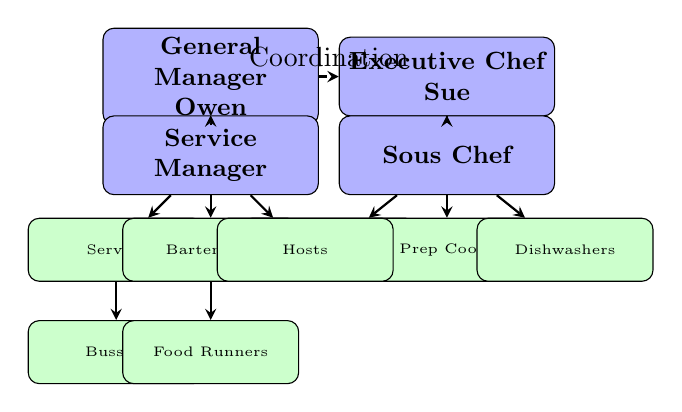
\begin{tikzpicture}[
    node distance=1.5cm,
    auto,
    manager/.style={rectangle, draw, fill=blue!30, text width=2.5cm, text centered, rounded corners, minimum height=1cm, font=\small\bfseries},
    staff/.style={rectangle, draw, fill=green!20, text width=2cm, text centered, rounded corners, minimum height=0.8cm, font=\tiny},
    arrow/.style={thick,->,>=stealth}
]
    % Management level
    \node [manager] (gm) {General Manager\\Owen};
    \node [manager, right of=gm, xshift=1.5cm] (chef) {Executive Chef\\Sue};
    
    % Second level
    \node [manager, below of=gm, yshift=0.5cm] (sm) {Service Manager};
    \node [manager, below of=chef, yshift=0.5cm] (sous) {Sous Chef};
    
    % Kitchen staff
    \node [staff, below of=sous, yshift=0.3cm, xshift=-1.5cm] (line1) {Line Cooks};
    \node [staff, below of=sous, yshift=0.3cm] (prep) {Prep Cooks};
    \node [staff, below of=sous, yshift=0.3cm, xshift=1.5cm] (dish) {Dishwashers};
    
    % Service staff
    \node [staff, below of=sm, yshift=0.3cm, xshift=-1.2cm] (server) {Servers};
    \node [staff, below of=sm, yshift=0.3cm] (bartender) {Bartenders};
    \node [staff, below of=sm, yshift=0.3cm, xshift=1.2cm] (host) {Hosts};
    \node [staff, below of=server, yshift=0.2cm] (busser) {Bussers};
    \node [staff, below of=bartender, yshift=0.2cm] (runner) {Food Runners};
    
    % Arrows
    \draw [arrow] (gm) -- (sm);
    \draw [arrow] (chef) -- (sous);
    \draw [arrow] (sous) -- (line1);
    \draw [arrow] (sous) -- (prep);
    \draw [arrow] (sous) -- (dish);
    \draw [arrow] (sm) -- (server);
    \draw [arrow] (sm) -- (bartender);
    \draw [arrow] (sm) -- (host);
    \draw [arrow] (server) -- (busser);
    \draw [arrow] (bartender) -- (runner);
    
    % Horizontal connection
    \draw [arrow, dashed] (gm) -- node [above] {Coordination} (chef);
\end{tikzpicture}
\caption{Restaurant Organizational Structure}
\label{fig:org_structure}
\end{figure}

\subsubsection{Management Team}
\begin{itemize}
    \item \textbf{General Manager} (Owen): Overall operations, financials, strategy
    \item \textbf{Executive Chef} (Sue): Kitchen operations, menu, food quality
    \item \textbf{Service Manager}: Front of house operations, guest relations
    \item \textbf{Sous Chef}: Kitchen management, training, execution
\end{itemize}

\subsubsection{Kitchen Staff}
\begin{itemize}
    \item Line cooks (hot line, cold line)
    \item Prep cooks
    \item Dishwashers
\end{itemize}

\subsubsection{Service Staff}
\begin{itemize}
    \item Servers
    \item Bartenders
    \item Hosts
    \item Bussers
    \item Food runners
\end{itemize}

\subsection{Job Descriptions | 工作描述 | Stellenbeschreibungen}

Clear job descriptions help attract the right candidates:

\subsubsection{Elements of Job Descriptions}
\begin{itemize}
    \item Job title and department
    \item Reports to (supervisor)
    \item Job summary
    \item Key responsibilities
    \item Required qualifications
    \item Preferred qualifications
    \item Physical requirements
    \item Schedule expectations
    \item Compensation range
\end{itemize}

\section{Recruitment Strategies | 招聘策略 | Rekrutierungsstrategien}

\subsection{Recruitment Channels | 招聘渠道 | Rekrutierungskanäle}

Sue and Owen used multiple channels to find candidates:

\subsubsection{Internal Methods}
\begin{itemize}
    \item Employee referrals (often best candidates)
    \item Promotions from within
    \item Internal job postings
\end{itemize}

\subsubsection{External Methods}
\begin{itemize}
    \item Online job boards (Indeed, LinkedIn, industry-specific)
    \item Social media (Facebook, Instagram)
    \item Culinary schools and hospitality programs
    \item Job fairs
    \item Industry associations
    \item Walk-in applications
    \item Competitor recruitment (ethical approach)
\end{itemize}

\subsection{Employer Branding | 雇主品牌 | Arbeitgebermarke}

Building a reputation as a great place to work:
\begin{itemize}
    \item Positive workplace culture
    \item Competitive compensation
    \item Growth opportunities
    \item Training and development
    \item Work-life balance (where possible)
    \item Community involvement
\end{itemize}

\section{The Hiring Process | 招聘流程 | Einstellungsprozess}

\subsection{Application Review | 申请审查 | Bewerbungsprüfung}

\begin{itemize}
    \item Review applications for basic qualifications
    \item Look for relevant experience
    \item Check for gaps or red flags
    \item Note any special skills or certifications
\end{itemize}

\subsection{Interview Process | 面试流程 | Interviewprozess}

\subsubsection{Phone Screening}
\begin{itemize}
    \item Initial qualification check
    \item Schedule availability
    \item Basic fit assessment
    \item 15-20 minutes
\end{itemize}

\subsubsection{In-Person Interviews}

Sue and Owen conducted structured interviews:

\begin{itemize}
    \item \textbf{Behavioral questions}: "Tell me about a time when..."
    \item \textbf{Situational questions}: "How would you handle..."
    \item \textbf{Technical questions}: Role-specific skills
    \item \textbf{Cultural fit}: Values alignment
    \item \textbf{Questions from candidate}: Engagement indicator
\end{itemize}

\subsubsection{Practical Assessments}

For kitchen positions:
\begin{itemize}
    \item Cooking demonstration
    \item Knife skills test
    \item Recipe execution
    \item Time management
\end{itemize}

For service positions:
\begin{itemize}
    \item Menu knowledge test
    \item Service scenario role-play
    \item Wine/spirits knowledge (if applicable)
    \item POS system familiarity
\end{itemize}

\subsection{Reference Checks | 背景调查 | Referenzprüfungen}

\begin{itemize}
    \item Contact previous employers
    \item Verify employment dates
    \item Ask about performance, reliability, teamwork
    \item Check for any concerns
\end{itemize}

\subsection{Background Checks | 背景调查 | Hintergrundprüfungen}

As legally permitted and appropriate:
\begin{itemize}
    \item Criminal background (if required by law)
    \item Employment verification
    \item Education verification (if relevant)
    \item Drug testing (if policy)
\end{itemize}

\subsection{Making the Offer | 发出录用通知 | Angebot machen}

\begin{itemize}
    \item Clear offer letter with:
    \begin{itemize}
        \item Position and title
        \item Start date
        \item Compensation (hourly rate or salary)
        \item Schedule expectations
        \item Benefits
        \item At-will employment statement
    \end{itemize}
    \item Set deadline for response
    \item Welcome and next steps
\end{itemize}

\section{Onboarding and Orientation | 入职与培训 | Einarbeitung und Orientierung}

\subsection{First Day Orientation | 第一天入职培训 | Orientierung am ersten Tag}

Sue and Owen created a comprehensive first-day experience:

\begin{itemize}
    \item Welcome and introductions
    \item Tour of facility
    \item Paperwork completion (I-9, W-4, policies)
    \item Overview of company culture and values
    \item Safety and security procedures
    \item Basic policies (attendance, dress code, breaks)
    \item Introduction to team
\end{itemize}

\subsection{Training Program | 培训计划 | Schulungsprogramm}

\subsubsection{Training Structure}

\begin{enumerate}
    \item \textbf{Orientation}: Company, culture, policies
    \item \textbf{Position-specific training}: Role requirements
    \item \textbf{Shadowing}: Learning from experienced staff
    \item \textbf{Supervised practice}: Hands-on with support
    \item \textbf{Evaluation}: Assessment of readiness
    \item \textbf{Independent work}: Gradual independence
\end{enumerate}

\subsubsection{Training Content}

\paragraph{For Kitchen Staff}
\begin{itemize}
    \item Food safety and sanitation
    \item Kitchen layout and equipment
    \item Menu knowledge
    \item Recipe execution
    \item Station procedures
    \item Quality standards
    \item Safety procedures
\end{itemize}

\paragraph{For Service Staff}
\begin{itemize}
    \item Service standards and steps
    \item Menu knowledge (ingredients, preparation, allergens)
    \item Wine and beverage knowledge
    \item POS system operation
    \item Table management
    \item Handling customer concerns
    \item Upselling techniques
\end{itemize}

\subsection{Training Methods | 培训方法 | Schulungsmethoden}

\begin{itemize}
    \item \textbf{Classroom training}: Policies, procedures, knowledge
    \item \textbf{Hands-on training}: Practical skills
    \item \textbf{Shadowing}: Observation and learning
    \item \textbf{Documentation}: Manuals, checklists, recipes
    \item \textbf{Videos}: Consistent demonstrations
    \item \textbf{Mentoring}: One-on-one guidance
\end{itemize}

\section{Ongoing Training and Development | 持续培训与发展 | Kontinuierliche Schulung und Entwicklung}

\subsection{Continuous Training | 持续培训 | Kontinuierliche Schulung}

Training doesn't end after onboarding:

\begin{itemize}
    \item \textbf{Menu changes}: New items, seasonal updates
    \item \textbf{Service improvements}: Refining standards
    \item \textbf{Safety updates}: New procedures, regulations
    \item \textbf{Skill development}: Advanced techniques
    \item \textbf{Cross-training}: Multiple positions
\end{itemize}

\subsection{Professional Development | 职业发展 | Berufliche Entwicklung}

Investing in employee growth:
\begin{itemize}
    \item Skill-building workshops
    \item Industry certifications
    \item Educational opportunities
    \item Career path discussions
    \item Leadership development
\end{itemize}

\section{Performance Management | 绩效管理 | Leistungsmanagement}

\subsection{Performance Standards | 绩效标准 | Leistungsstandards}

Clear expectations for all positions:
\begin{itemize}
    \item Quality standards
    \item Productivity expectations
    \item Attendance requirements
    \item Customer service standards
    \item Teamwork expectations
\end{itemize}

\subsection{Performance Reviews | 绩效评估 | Leistungsbeurteilungen}

Regular feedback and evaluation:
\begin{itemize}
    \item \textbf{Daily feedback}: Immediate, specific
    \item \textbf{Weekly check-ins}: Progress, concerns
    \item \textbf{Formal reviews}: Quarterly or semi-annual
    \item \textbf{360-degree feedback}: From peers, supervisors, customers
\end{itemize}

\subsection{Recognition and Rewards | 认可与奖励 | Anerkennung und Belohnungen}

\begin{itemize}
    \item \textbf{Verbal recognition}: Public acknowledgment
    \item \textbf{Employee of the month}: Recognition program
    \item \textbf{Performance bonuses}: Financial rewards
    \item \textbf{Career advancement}: Promotions
    \item \textbf{Special perks}: Meals, events, benefits
\end{itemize}

\section{Retention Strategies | 保留策略 | Bindungsstrategien}

\subsection{Why Employees Leave | 员工离职的原因 | Warum Mitarbeiter gehen}

Common reasons for turnover:
\begin{itemize}
    \item Low compensation
    \item Poor management
    \item Lack of growth opportunities
    \item Unfavorable work environment
    \item Scheduling issues
    \item Lack of recognition
\end{itemize}

\subsection{Retention Tactics | 保留策略 | Bindungsstrategien}

Sue and Owen focused on:

\begin{itemize}
    \item \textbf{Competitive compensation}: Market-rate pay, tips
    \item \textbf{Positive culture}: Respect, teamwork, fun
    \item \textbf{Growth opportunities}: Training, promotions
    \item \textbf{Flexible scheduling}: Where possible
    \item \textbf{Benefits}: Health insurance, paid time off
    \item \textbf{Recognition}: Appreciation and rewards
    \item \textbf{Communication}: Open, honest, regular
    \item \textbf{Work-life balance}: Reasonable hours, time off
\end{itemize}

\section{Workplace Culture | 工作场所文化 | Arbeitsplatzkultur}

\subsection{Building a Positive Culture | 建立积极文化 | Positive Kultur aufbauen}

\begin{itemize}
    \item \textbf{Clear values}: Define and communicate
    \item \textbf{Lead by example}: Management behavior
    \item \textbf{Respect}: For all team members
    \item \textbf{Teamwork}: Collaboration and support
    \item \textbf{Communication}: Open, honest, regular
    \item \textbf{Recognition}: Celebrate successes
    \item \textbf{Problem-solving}: Address issues promptly
    \item \textbf{Fun}: Enjoyable work environment
\end{itemize}

\subsection{Handling Conflict | 处理冲突 | Konflikte bewältigen}

\begin{itemize}
    \item Address issues promptly
    \item Listen to all parties
    \item Find solutions, not blame
    \item Document serious issues
    \item Follow progressive discipline when needed
    \item Maintain confidentiality
\end{itemize}

\section{Compliance and Legal Considerations | 合规与法律考虑 | Compliance und rechtliche Überlegungen}

\subsection{Labor Laws | 劳动法 | Arbeitsgesetze}

\begin{itemize}
    \item \textbf{Fair Labor Standards Act (FLSA)}: Minimum wage, overtime
    \item \textbf{Equal Employment Opportunity}: Non-discrimination
    \item \textbf{Family and Medical Leave Act (FMLA)}: Leave requirements
    \item \textbf{Occupational Safety and Health Act (OSHA)}: Workplace safety
    \item \textbf{State and local laws}: Additional requirements
\end{itemize}

\subsection{Employment Practices | 雇佣实践 | Beschäftigungspraktiken}

\begin{itemize}
    \item Proper classification (exempt vs. non-exempt)
    \item Accurate time tracking
    \item Proper break and meal periods
    \item Tip pooling and distribution rules
    \item Documentation of performance issues
    \item Termination procedures
\end{itemize}

\section{Scheduling and Labor Costs | 排班与人工成本 | Zeitplanung und Arbeitskosten}

\subsection{Scheduling Best Practices | 排班最佳实践 | Best Practices für die Zeitplanung}

\begin{itemize}
    \item Forecast sales and labor needs
    \item Schedule based on business patterns
    \item Consider employee preferences (where possible)
    \item Adequate coverage without overstaffing
    \item Cross-training for flexibility
    \item Advance notice (2 weeks minimum)
\end{itemize}

\subsection{Labor Cost Management | 人工成本管理 | Arbeitskostenmanagement}

\begin{itemize}
    \item Target labor cost percentage (typically 25-35\% of sales)
    \item Monitor daily and weekly
    \item Adjust schedules based on business
    \item Optimize productivity
    \item Balance service quality with costs
\end{itemize}

\trilingualsection{Key Takeaways}{关键要点}{Wichtige Erkenntnisse}{}

\begin{itemize}
    \item People are the restaurant's greatest asset
    \item Clear job descriptions attract the right candidates
    \item Comprehensive training ensures quality and consistency
    \item Ongoing development retains and motivates staff
    \item Positive culture improves retention and performance
    \item Performance management maintains standards
    \item Compliance protects the business and employees
    \item Effective scheduling balances service and costs
\end{itemize}

With a strong team in place, Sue and Owen's restaurant had the human foundation for success. However, financial management would determine whether the business could thrive long-term. The next chapter explores the critical financial aspects of restaurant operations.
